\begin{problem}{전생했더니 슬라임 연구자였던 건에 대하여 (Hard)}{standard input}{standard output}

안녕? 내 이름은 ntopia!

나는 원래 지구에 살고있던 평범한 20대 청년이었어. 어느날 길을 걷다가 괴한의 칼에 찔려
죽어버렸어. 그런데 이게 무슨 일이람! 정신을 차려보니 이세계에 떨어져버렸지 뭐야.
여기에서 나는 슬라임을 전문으로 연구하는 슬라임 연구자가 되어버린 것 같아.
나는 지금 아주 중요한 연구를 진행하고 있어. 이 연구가 성공하면 나는 내가 살던 세계로
돌아갈 수 있게 될거야. 이 연구를 도와주지 않겠니?

이 곳의 슬라임은 모두 슬라임 에너지라는 것을 갖고 있고 그 양은 2 이상의 자연수로 표현돼.
나는 슬라임을 합성했을 때 슬라임 에너지가 어떻게 변화하는지에 대해 연구하고 있어.

슬라임 합성 과정은 2마리를 합성해서 1마리를 만들어내는 식으로 이루어져.
$A$만큼의 슬라임 에너지를 갖고 있는 슬라임과 $B$만큼의 슬라임 에너지를 갖고 있는
슬라임이 있었다고 해보자. 이 슬라임 2마리를 합성하면
슬라임 에너지가 $A * B$ 인 슬라임을 만들 수 있어.

그리고 슬라임 합성 기술이 아직 완벽하지 않아서 슬라임을 합성할 때마다
크나큰 전기 에너지를 필요로 해. 구체적으로,
$A$만큼의 슬라임 에너지를 갖고 있는 슬라임과 $B$만큼의 슬라임 에너지를 갖고 있는 슬라임을
합성하려면 $A * B$ 만큼의 전기 에너지가 필요해.

\begin{center}
  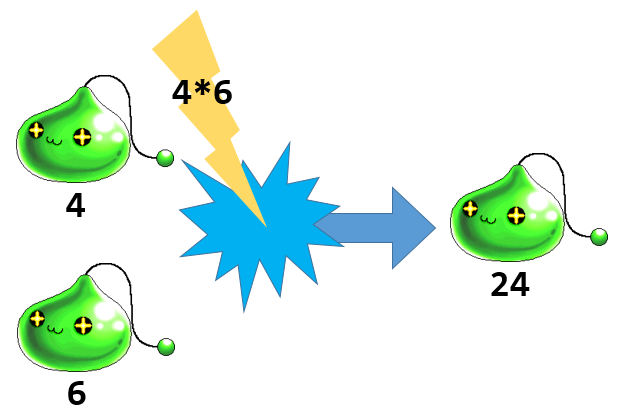
\includegraphics[width=0.7\textwidth]{slime_compose.png}
  \begin{figure}[!h]
  \captionsetup{labelformat=empty,justification=centering}
  \caption{에너지가 4인 슬라임과 에너지가 6인 슬라임을 합성한 모습. 4*6의 전기 에너지를 사용해 슬라임 에너지가 24인 슬라임이 합성되었다.}
  \end{figure}
\end{center}

나에겐 지금 $N$마리의 슬라임이 있어. 이 슬라임들을 모두 적절히 합성해서
1마리의 슬라임으로 만들려고 해. 그런데 내가 소속된 연구소에서
각 합성 단계마다 필요한 전기 에너지들을 모두 곱한 값을 나에게 비용으로
청구하겠다고 했지 뭐야. 결국 이 값이 최소가 되도록 합성을 적절히 수행하는 것이 내 연구의 목표야.

내 연구를 도와줘! 부탁이야!!

\InputFile
첫 번째 줄에 테스트 케이스의 수 $T$ 가 주어지고, 이어서 $T$ 개의 테스트 케이스가 주어진다.

각 테스트 케이스의 첫 번째 줄에는 슬라임의 수 $N$ ($2 \le N \le 60$)이 주어지고, 두 번째 줄에는 $N$ 개의 자연수가 주어진다. $i$번째 자연수 $C_i$ ($2 \le C_i \le 10^{18}$) 는 $i$번째 슬라임의 슬라임 에너지를 나타낸다. 끝까지 합성하고 난 후에 생기는 슬라임의 에너지의 양이 $10^{18}$ 이하라는 것이 보장된다.

모든 테스트 케이스에 대한 $N$ 의 총합이 $1,000,000$을 넘지 않음이 보장된다.

\OutputFile
각 테스트 케이스마다 슬라임을 끝까지 합성했을 때 청구될 비용의 최소값을 $1,000,000,007$로 나눈 나머지를 출력한다.

\Example

\begin{example}
\exmp{1
5
3 10 2 8 14}{270950400}%
\end{example}

\end{problem}
